\documentclass[12pt]{article}

\usepackage[margin=1in]{geometry} 
\usepackage{amsmath,amsthm,amssymb}
\usepackage{graphicx}
\usepackage{booktabs}
\usepackage{caption}
\captionsetup{font=small}
\usepackage{subcaption} 
\usepackage{hyperref}

\newcommand{\N}{\mathbb{N}}
\newcommand{\Z}{\mathbb{Z}}

\newenvironment{solution}{\begin{proof}[Solution]}{\end{proof}}

\begin{document}

% --------------------------------------------------------------
%                         Title
% --------------------------------------------------------------

\begin{titlepage}
    \centering
    \vspace*{\fill}
    {\LARGE Software Development Oriented to ML \par}
    {\LARGE Garbage Classifier \par}
    \vspace{1cm}
    {\large Melchor Lafuente\par}
    {\large Iker Jauregui \par}
    \vspace*{\fill}
\end{titlepage}

\newpage

\section{Introduction}
The \textbf{GarbageClassifier} project is a deep learning approach to automatically classify images of common waste into six categories: cardboard, glass, metal, paper, plastic, and trash. The system leverages \textbf{PyTorch Lightning} for structured training and organization of the deep learning pipeline, using \textbf{ResNet18} as the backbone model.\\

The project dataset originates from the \href{https://www.kaggle.com/datasets/zlatan599/garbage-dataset-classification?resource=download}{Garbage Classification Dataset on Kaggle} and has been reduced in size for experimentation purposes. A sample dataset was created for rapid prototyping, containing 100 images per class (90 for training and 10 for testing).

\section{Exploratory Data Analysis (EDA)}
EDA was performed to understand the dataset characteristics and to guide model development. Key observations include:

\begin{itemize}
    \item The classes are relatively balanced as shown in figure \ref{fig:class_distribution}.
    \item All images are 256$\times$256 pixels.
    \item Class prototypes, calculated as the mean image per class, revealed distinctive visual characteristics:
    \begin{itemize}
        \item \textbf{Cardboard:} Brown-orange tones.
        \item \textbf{Plastic:} Blue-gray hues.
        \item \textbf{Glass:} Greenish tint, with bottle shape visible.
        \item \textbf{Metal:} Dark gray, with central square-like pattern.
        \item \textbf{Trash:} Brown-gray tones, diverse textures.
        \item \textbf{Paper:} Uniform light gray.
    \end{itemize}
    \item Confusion is likely between metal, plastic, and paper classes due to visual similarity, as highlighted by the prototypes.
\end{itemize}

\begin{figure}[h!]
    \centering
    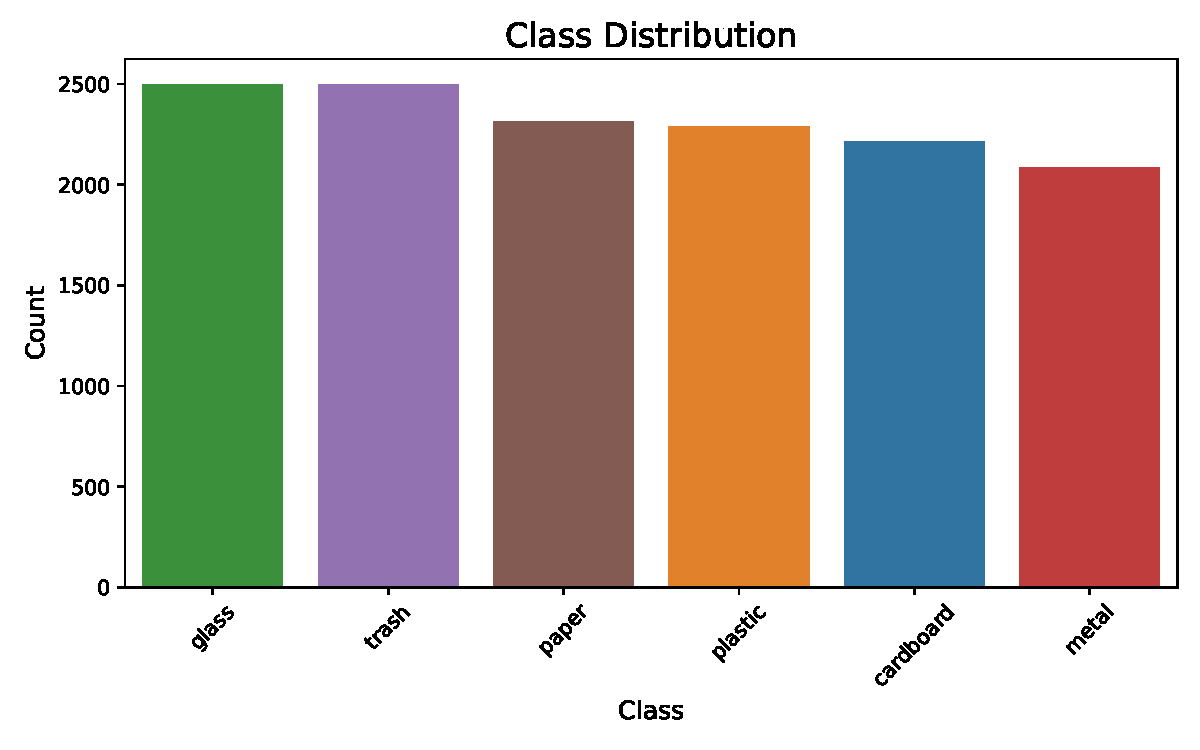
\includegraphics[width=0.4\textwidth]{figures/EDA/class_distribution.pdf}
    \caption{Number of samples per class.}
    \label{fig:class_distribution}
\end{figure}

\newpage
\begin{figure}[h!]
    \centering
    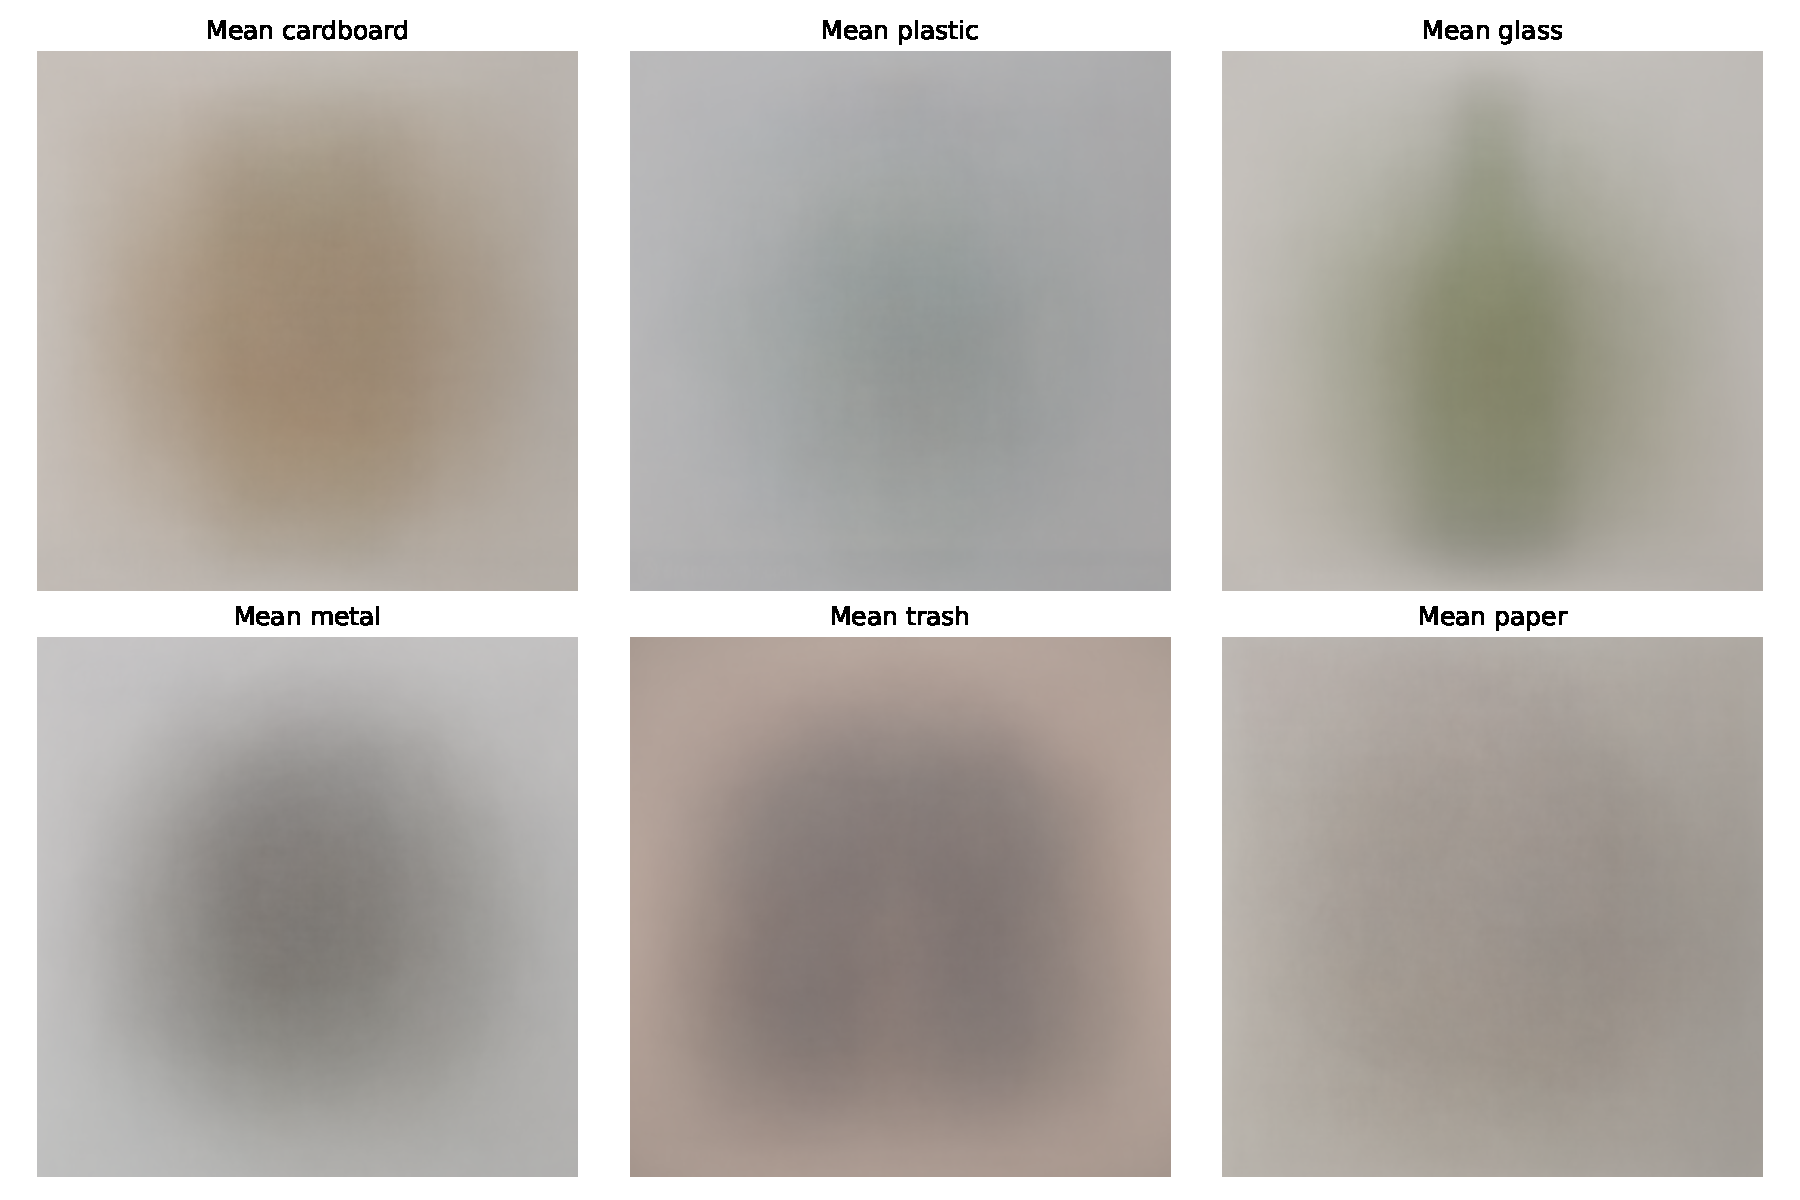
\includegraphics[width=0.8\textwidth]{figures/EDA/class_prototypes_mean.pdf}
    \caption{Mean images per class highlighting prototypical characteristics.}
    \label{fig:mean_images}
\end{figure}

\begin{figure}[h!]
    \centering
    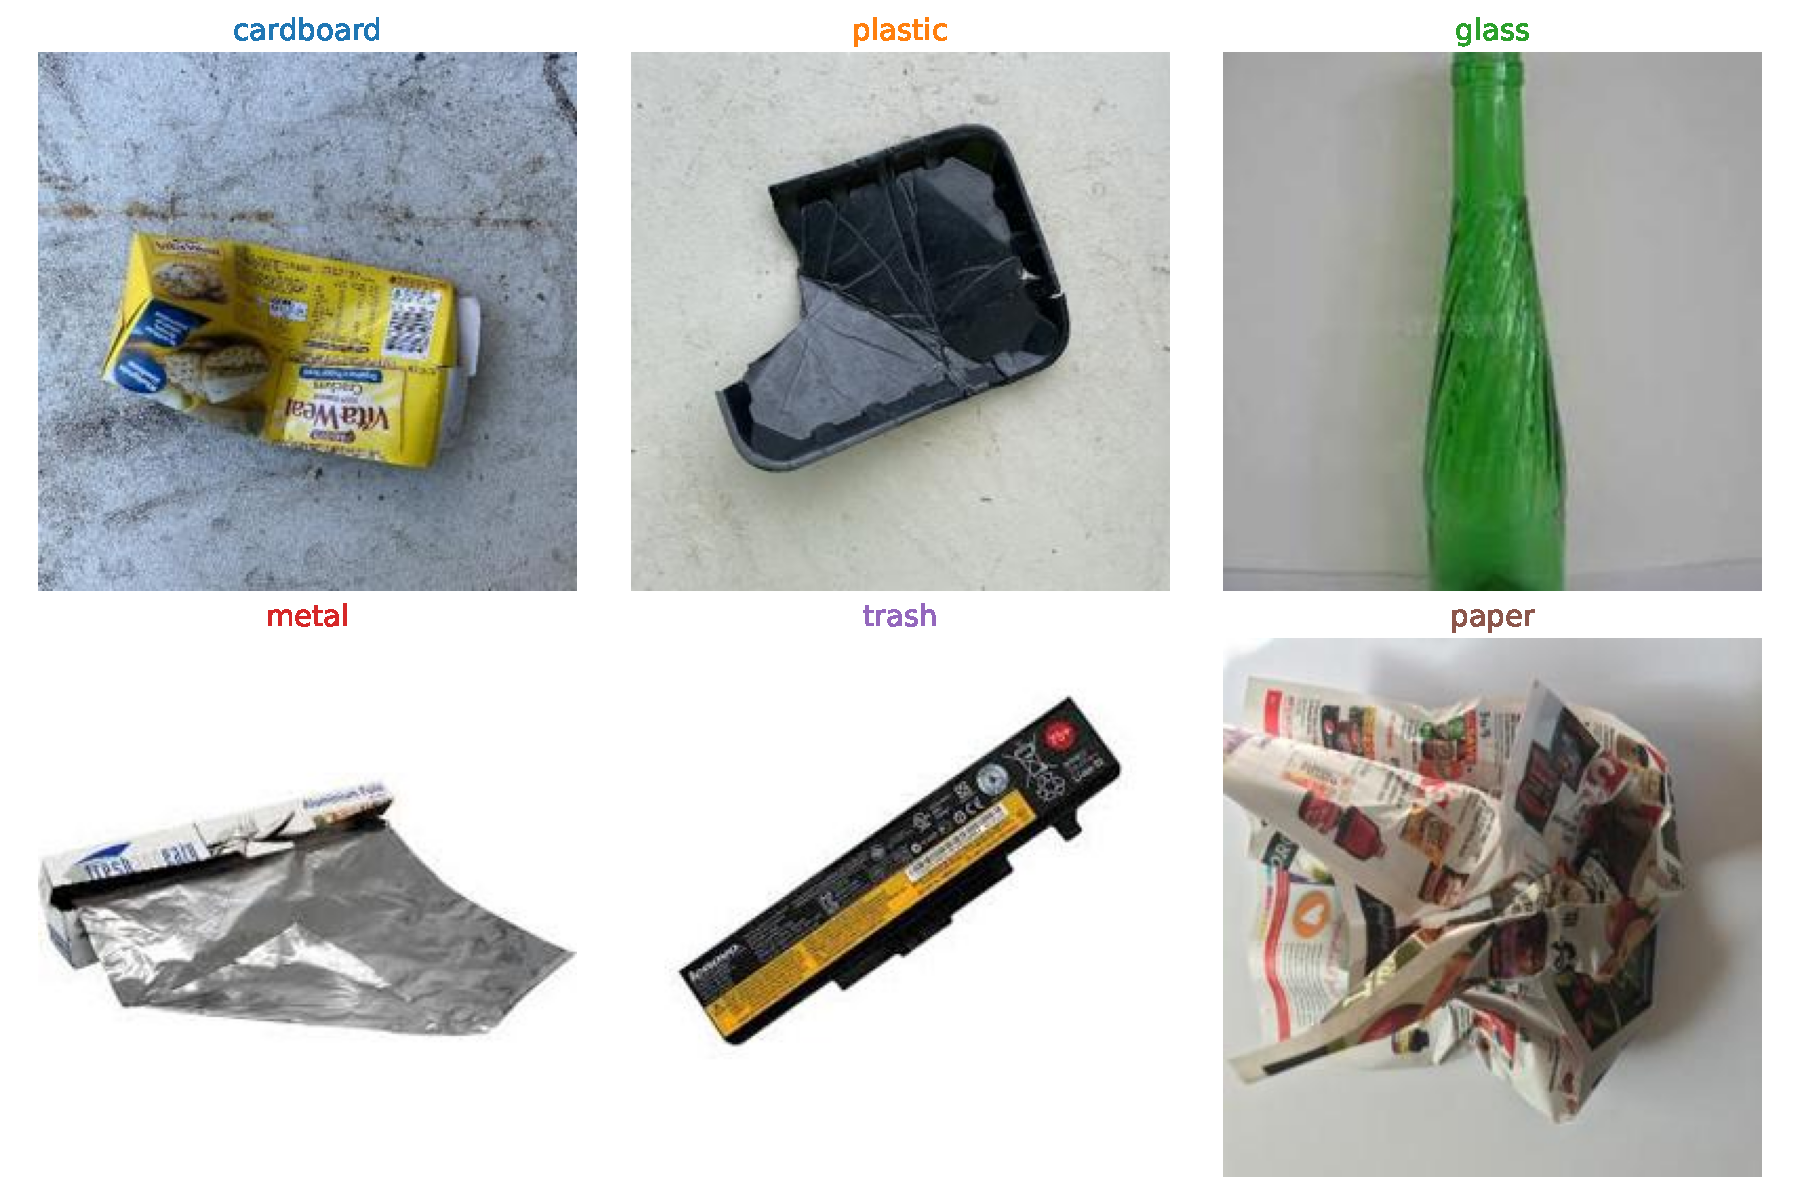
\includegraphics[width=0.8\textwidth]{figures/EDA/random_examples_per_class.pdf}
    \caption{Random samples per class.}
    \label{fig:rand_samples}
\end{figure}

\newpage
\section{Model Training and Performance}
The \textbf{ResNet18}-based \texttt{GarbageClassifier} was trained for 10 epochs on the reduced dataset. Performance metrics were evaluated on training and testing subsets.

\subsection{Loss and Accuracy Curves}
The training and validation loss curves indicate that the model has not fully converged, suggesting potential improvements with additional epochs. Validation accuracy shows room for enhancement as well.

\begin{figure}[h!]
    \centering
    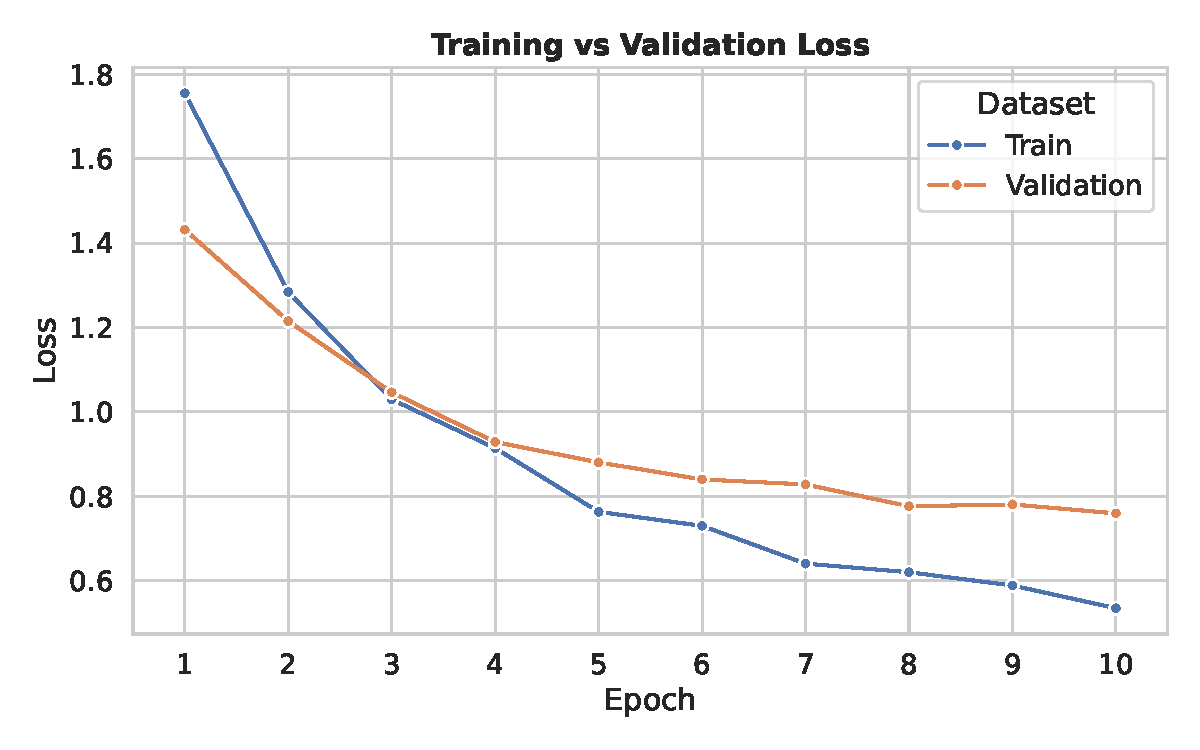
\includegraphics[width=0.45\textwidth]{figures/performance/train_vs_val_loss.pdf}
    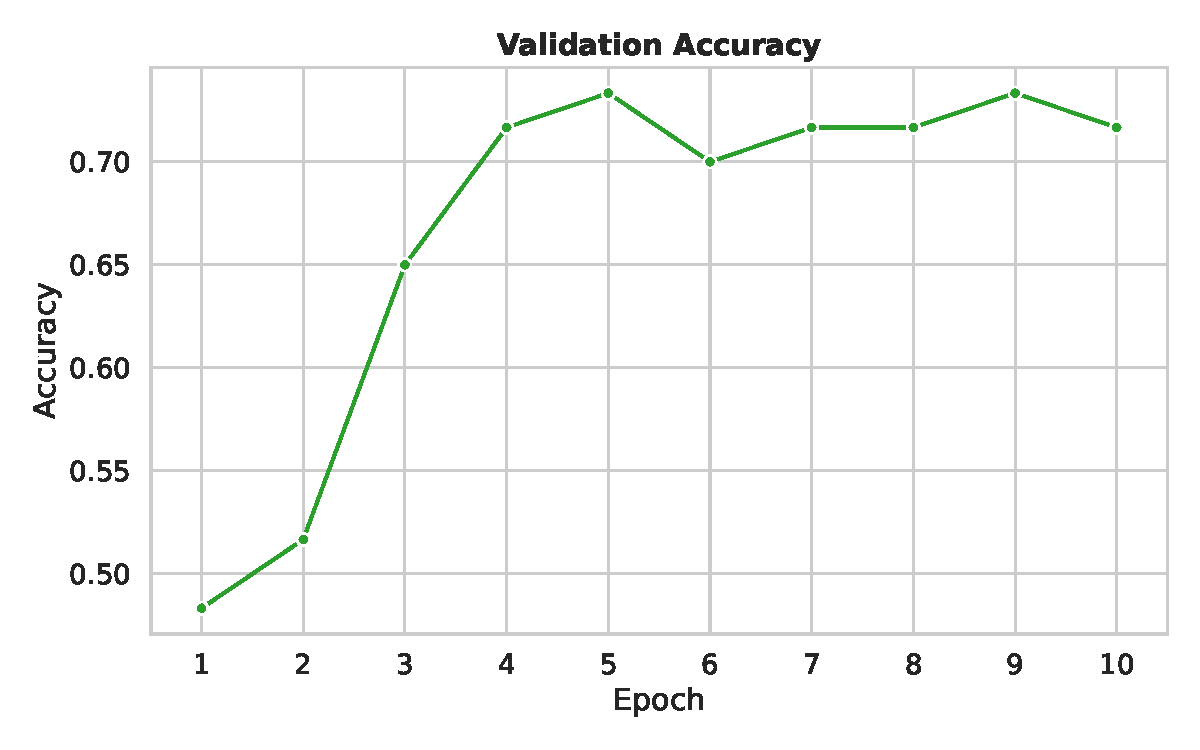
\includegraphics[width=0.45\textwidth]{figures/performance/val_acc.pdf}
    \caption{Left: Training vs validation loss. Right: Validation accuracy.}
    \label{fig:loss_acc}
\end{figure}

\subsection{Confusion Matrices}
Confusion matrices reveal that most misclassifications occur among \textbf{metal, paper, and plastic}, aligning with the visual similarities observed in the EDA. 

\begin{figure}[h!]
    \centering
    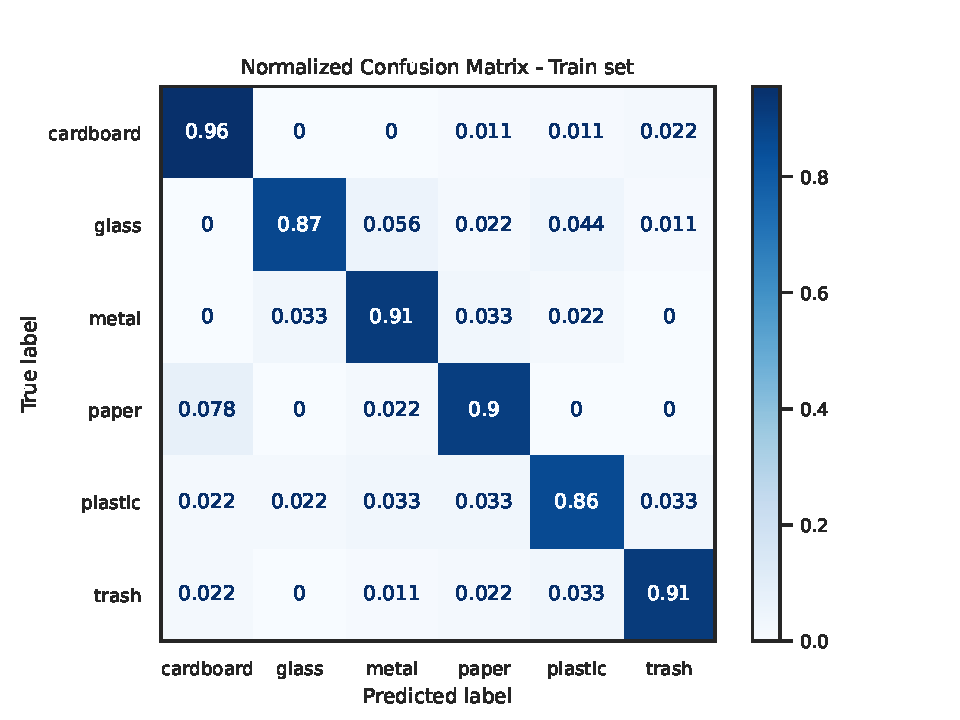
\includegraphics[width=0.45\textwidth]{figures/performance/confussion_mat_train_norm.pdf}
    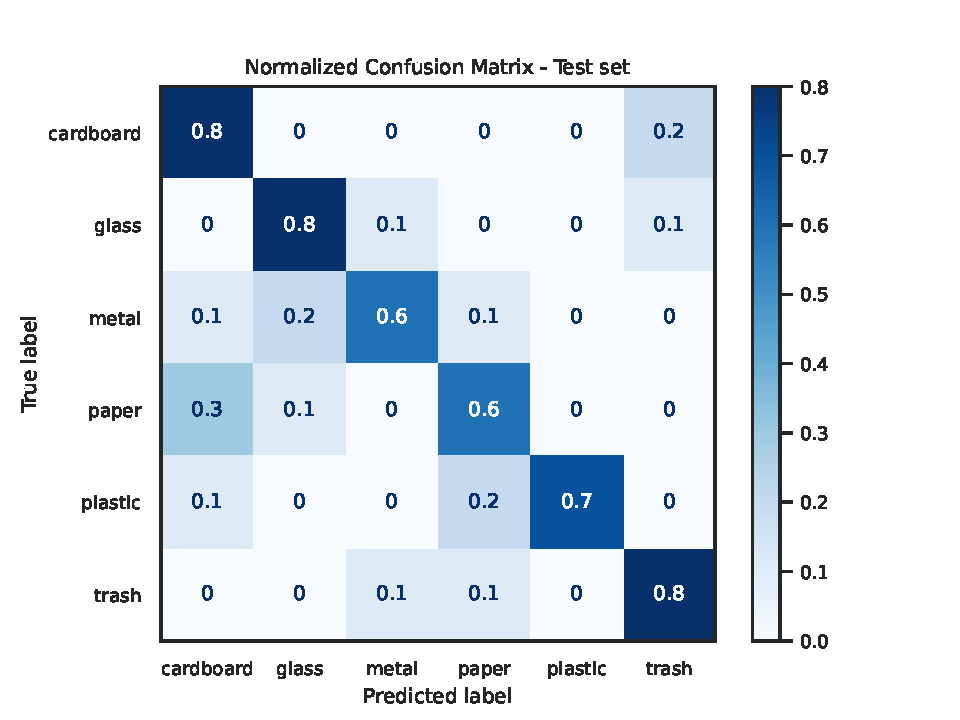
\includegraphics[width=0.45\textwidth]{figures/performance/confussion_mat_test_norm.pdf}
    \caption{Normalized confusion matrices for training (left) and test (right) sets.}
    \label{fig:confusion}
\end{figure}

\newpage
\subsection{Calibration Curves}
Calibration curves suggest that the model is not very well calibrated except for the \textbf{paper} class.

\begin{figure}[h!]
    \centering
    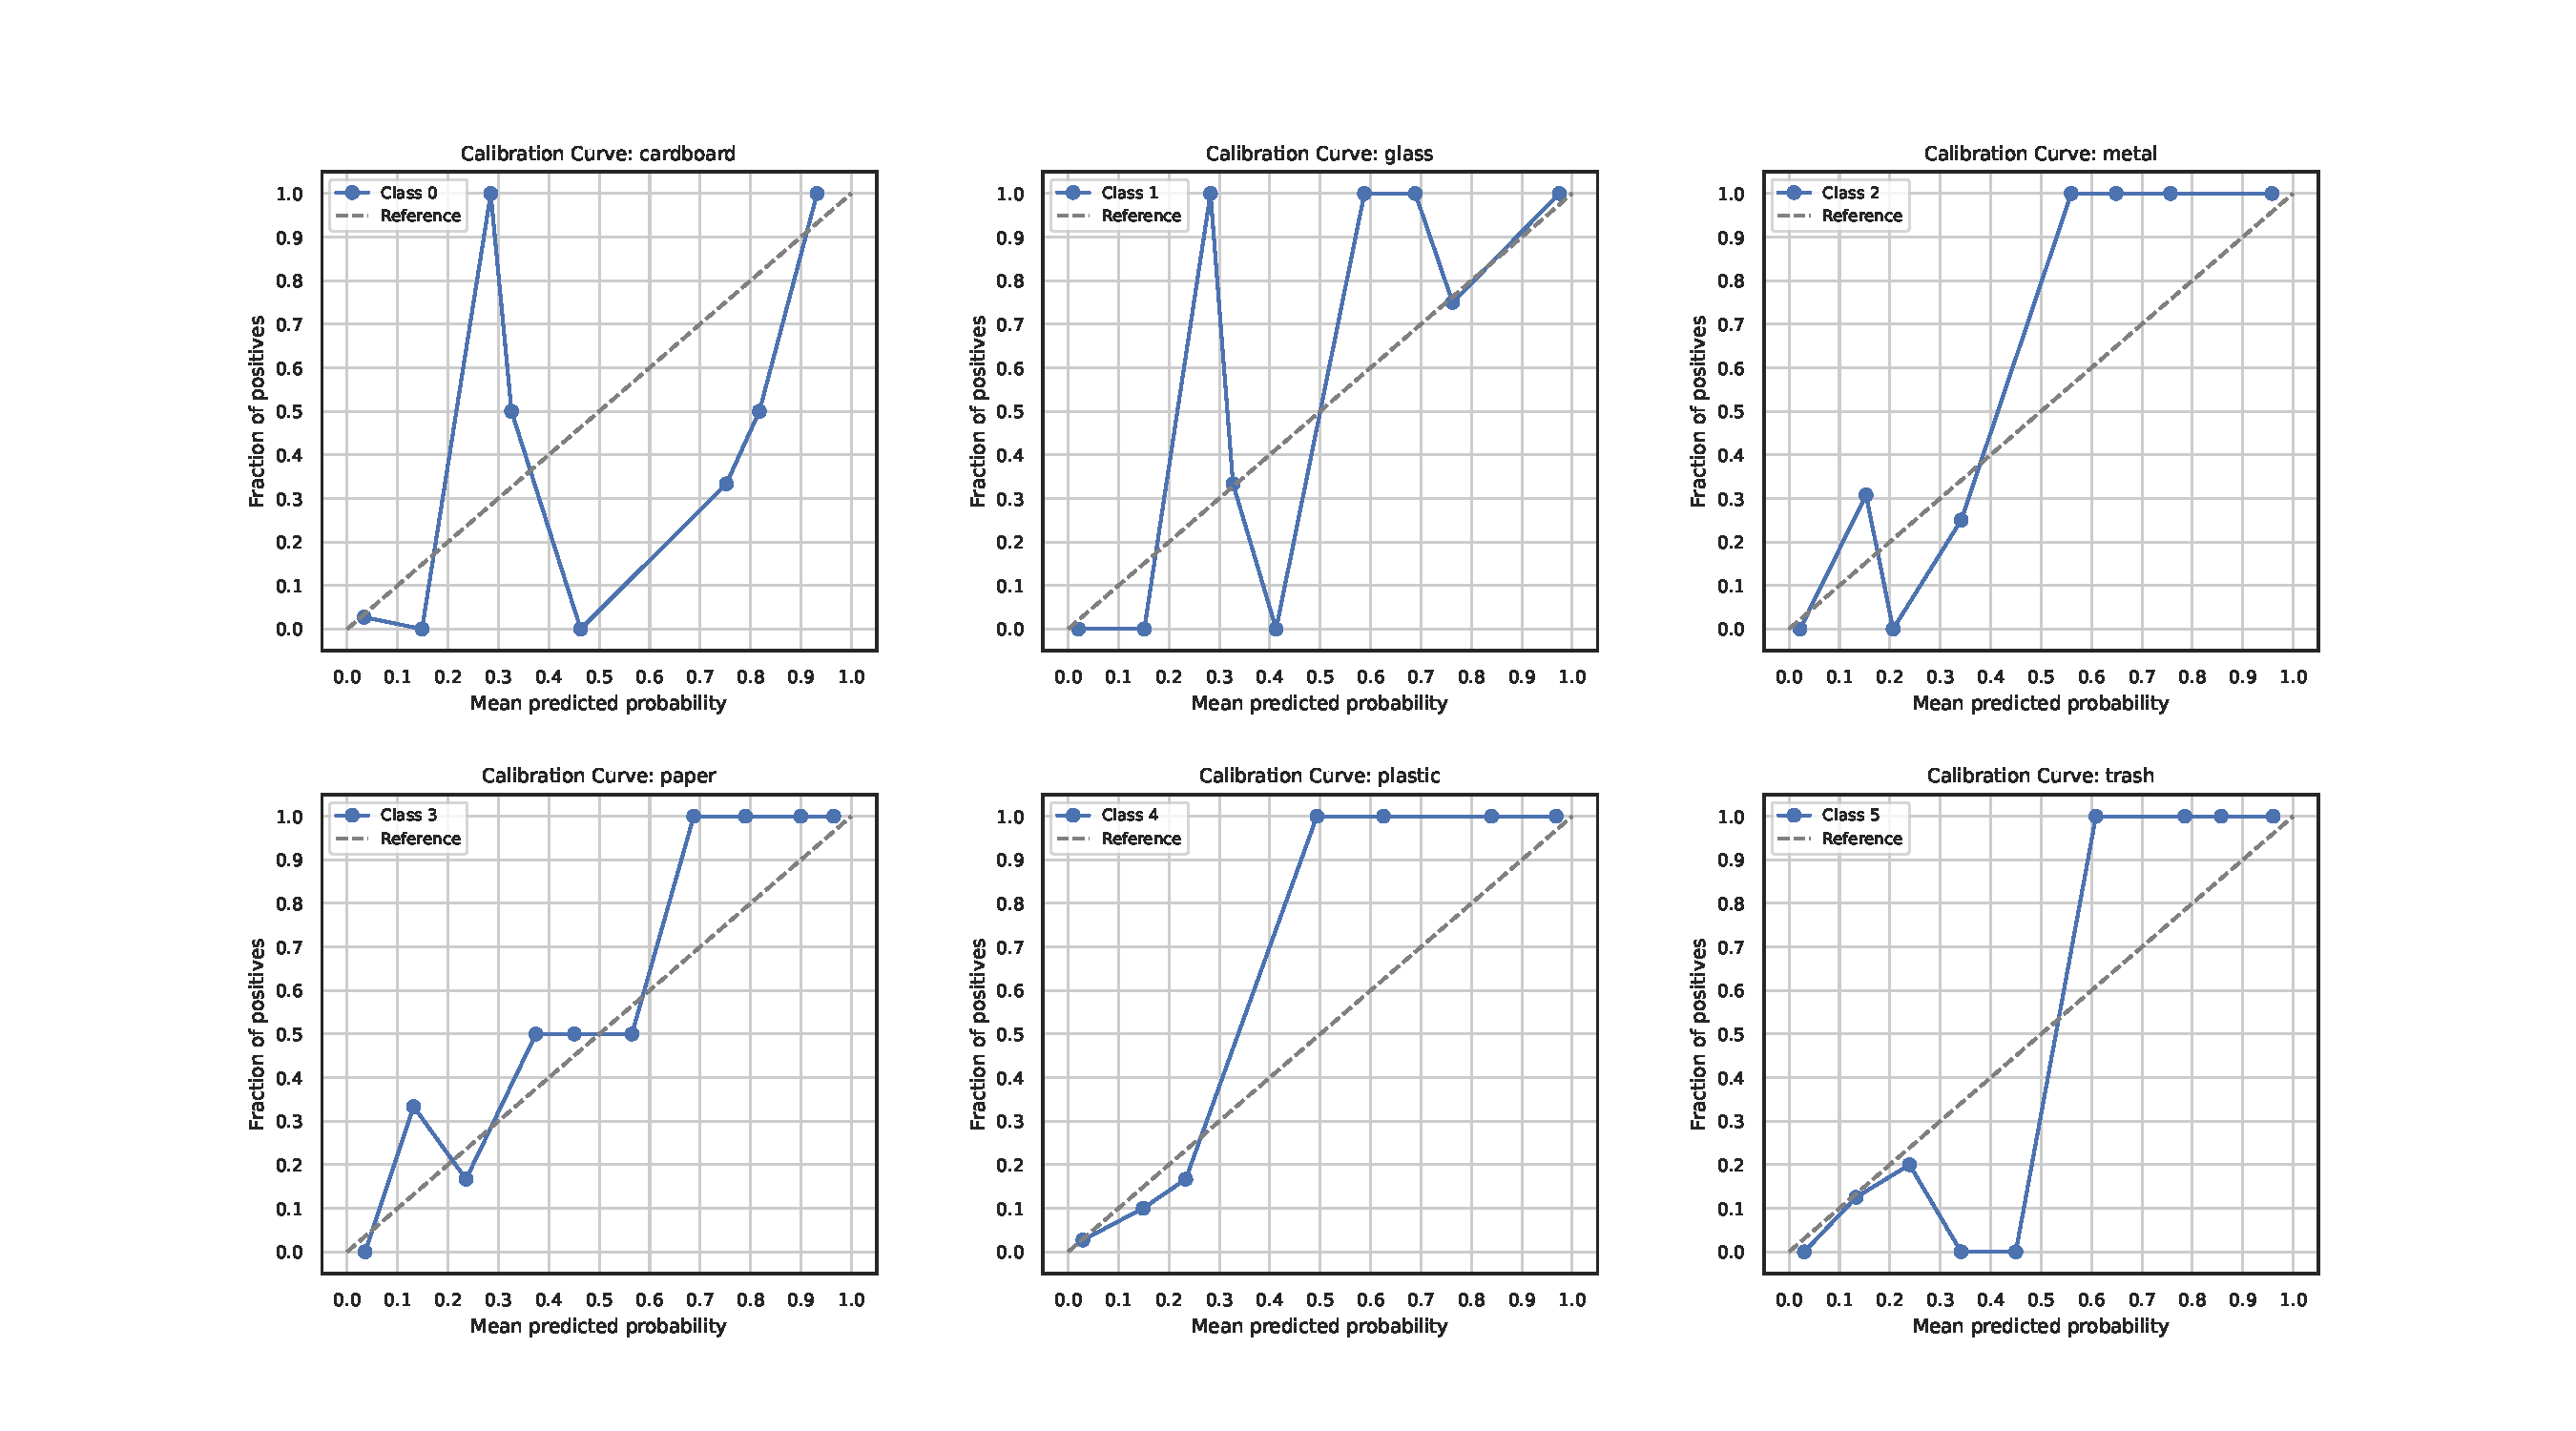
\includegraphics[width=0.8\textwidth]{figures/performance/calibration_curves.pdf}
    \caption{Calibration curves per class.}
    \label{fig:calibration}
\end{figure}

\subsection{Error Analysis}
Examining the samples with the lowest confidence we can try to think why is the model making bad decisions:
\begin{itemize}
    \item The model relies too heavily on color.
    \item The red underwear and blue masks are completely unrelated to each other and to the other trash examples, which confirms that the model struggles because there is no clear pattern.
\end{itemize}

\begin{figure}[h!]
    \centering
    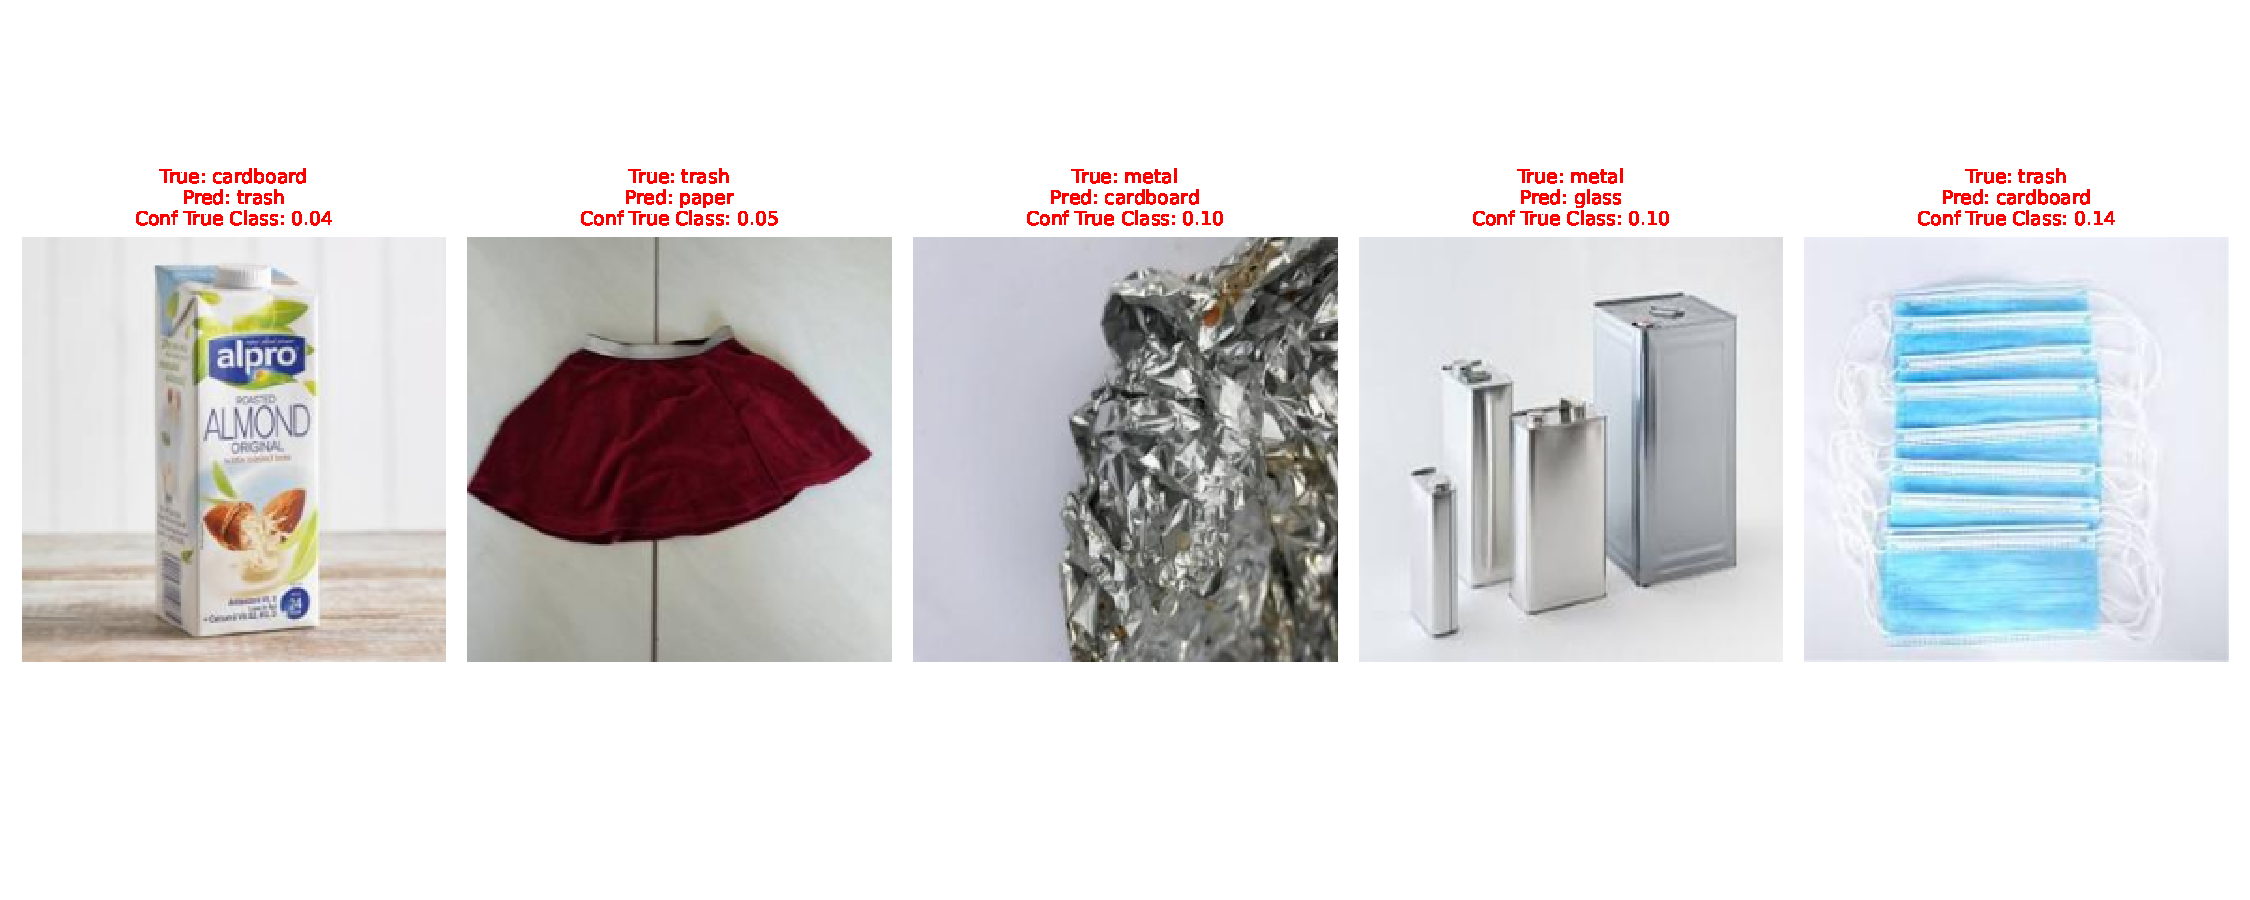
\includegraphics[width=0.7\textwidth]{figures/worst_classified_test_samples.pdf}
    \caption{Worst classified test samples, indicating challenging textures and ambiguous objects.}
    \label{fig:worst_samples}
\end{figure}

\newpage
\section{Conclusions}
The EDA helped identify potential sources of confusion among classes and informed model evaluation. Key takeaways include:

\begin{itemize}
    \item The ResNet18-based model shows promising initial results but requires more training data and epochs to fully converge.
    \item Misclassifications mostly involve metal, plastic, and paper, as predicted by EDA prototypes.
    \item Advanced data augmentation or input transformations could improve feature extraction for challenging textures and colors.
    \item A rejection-class approach may help address the heterogeneous nature of the trash class.
\end{itemize}

Future work should focus on scaling the dataset, enhancing augmentation strategies, and exploring more complex architectures or training paradigms to improve robustness and generalization.

\end{document}